\providecommand{\home}{../../..}
\documentclass[\home/main.tex]{subfiles}
\usetikzlibrary[arrows,snakes,backgrounds]

\begin{document}

\def\layersep{1.5cm}

\newsavebox{\neuralnetworkBox}
\sbox{\neuralnetworkBox}{%
    \begin{tikzpicture}[
            shorten >=1pt,->,
            draw=black!50,
            node distance=\layersep,
            every pin edge/.style={<-,shorten <=1pt},
            neuron/.style={circle,fill=black!25,minimum size=17pt,inner sep=0pt},
            input neuron/.style={neuron, fill=green!50},
            output neuron/.style={neuron, fill=red!50},
            hidden neuron/.style={neuron, fill=blue!50},
            annot/.style={text width=4em, text centered}
        ]
        % set number of hidden layers
        \newcommand\Ninputs{3}
        \newcommand\Nhidden{2}
        \newcommand\Noutputs{3}

        % Draw the input layer nodes
        \foreach \name / \y in {1,...,\Ninputs}
        % This is the same as writing \foreach \name / \y in {1/1,2/2,3/3,4/4}
        % \node[input neuron, pin=left:Input \#\y] (I-\name) at (0,-\y) {};
        \node[input neuron] (I-\name) at (0,-\y) {};

        % Draw the hidden layer nodes
        \foreach \N in {1,...,\Nhidden} {
                \foreach \y in {1,...,5} {
                        \path[yshift=0.5cm]
                        node[hidden neuron] (H\N-\y) at (\N*\layersep,-\y cm) {};
                    }
                \node[annot,above of=H\N-1, node distance=1cm] (hl\N) {};
            }

        % Draw the output layer node
        % \node[output neuron,pin={[pin edge={->}]right:Output}, right of=H\Nhidden-3] (O) {};
        \node[output neuron, right of=H\Nhidden-3] (O) {};

        % Connect every node in the input layer with every node in the hidden layer.
        \foreach \source in {1,...,4}
        \foreach \dest in {1,...,5}
        \path (I-\source) edge (H1-\dest);

        % connect all hidden stuff
        \foreach [remember=\N as \lastN (initially 1)] \N in {2,...,\Nhidden}
        \foreach \source in {1,...,5}
        \foreach \dest in {1,...,5}
        \path (H\lastN-\source) edge (H\N-\dest);

        % Connect every node in the hidden layer with the output layer
        \foreach \source in {1,...,5}
        \path (H\Nhidden-\source) edge (O);

        % Annotate the layers
        % \node[annot,left of=hl1] {Inputs};
        % \node[annot,right of=hl\Nhidden] {Outputs};

    \end{tikzpicture}%
}

\newcommand{\scaledMLP}[2]{\resizebox{#1}{#2}{\usebox{\neuralnetworkBox}}}
\newcommand{\scaledMLPwidth}[1]{\resizebox{#1}{!}{\usebox{\neuralnetworkBox}}}
\newcommand{\scaledMLPratio}[1]{\resizebox{!}{#1}{\usebox{\neuralnetworkBox}}}

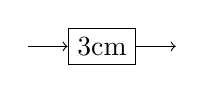
\begin{tikzpicture}
    \draw (0,0) node[draw](filt){\scaledMLPratio{3cm}};
    \draw [<-] (filt.west) -- ++(-0.5,0);
    \draw [->] (filt.east) -- ++(0.5,0);
\end{tikzpicture}

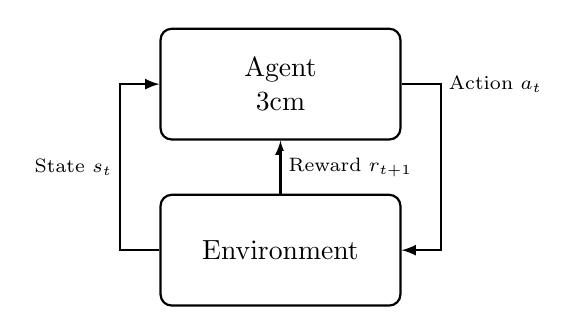
\begin{tikzpicture}[node distance = 6em, auto, thick]
    \tikzset{
        block/.style={
                rectangle, draw, text width=8em, text centered, rounded corners, minimum height=4em
            },
        descr/.style={
                fill=white,
                inner sep=2.5pt
            },
        connector/.style={
                -latex,
                font=\scriptsize
            },
        % Based on https://tex.stackexchange.com/questions/50780/arrows-at-right-angles-on-a-tikzpicture-matrix
        rectangle connector/.style={
                connector,
                to path={(\tikztostart) -- ++(#1,0pt) |- (\tikztotarget)  \tikztonodes },
                pos=0.25
            },
        rectangle connector/.default=-2cm,
        straight connector/.style={
                connector,
                to path=--(\tikztotarget) \tikztonodes
            }
    }

    \node[block]        (agent)                                           {Agent\\\scaledMLPwidth{3cm}};
    \node[block]        (env)       [below of=agent]                      {Environment};

    % Don't delete this, this is how I did it manually without \tikztonodes macro magic 
    % \draw [->] (env) to node [auto, swap] {Reward} (agent);
    % \draw [->] (env.west) -- ++(-0.5,0) |- node[pos=0.25] {State} (agent.west); % first go left a bit, then go vertical and horizontal to agent node while putting a label with name "State" on it
    % \draw [->] (agent.east) --++(0.5,0) |- node[pos=0.25] {Action}               (env.east);

    \draw [straight connector] (env) to node [descr, swap] {Reward $r_{t+1}$} (agent);
    \draw [rectangle connector=0.5cm] (agent.east) to node[descr, pos=0] {Action $a_{t}$} (env.east);
    \draw [rectangle connector=-0.5cm] (env.west) to node[descr] {State $s_{t}$} (agent.west);


\end{tikzpicture}
\end{document}
